\chapter{Multiparty secure computation I: Definition and
Honest-But-Curious to Malicious complier}\label{sfeonechap}

Wikipedia \href{https://en.wikipedia.org/wiki/Cryptography}{defines}
cryptography as ``the practice and study of techniques for secure
communication in the presence of third parties called adversaries''.
However, I think a better definition would be:

\begin{quote}
\emph{Cryptography is about replacing trust with mathematics.}
\end{quote}

After all, the reason we work so hard in cryptography is because a lack
of trust. We wouldn't need encryption if Alice and Bob could be
guaranteed that their communication, despite going through wireless and
wired networks controlled and snooped upon by a plethora of entities,
would be as reliable as if it has been hand delivered by a
letter-carrier as reliable as
\href{http://old.iolaregister.com/Local\%20News/Stories/Weatherwontstopcarriers.html}{Patti
Whitcomb}, as opposed to the nosy Eve who might look in the messages, or
the malicious Mallory, who might tamper with them. We wouldn't need zero
knowledge proofs if Vladimir could simply say ``trust me Barack, this is
an authentic nuke''. We wouldn't need electronic signatures if we could
trust that all software updates are designed to make our devices safer
and not, to pick a random example, to turn our phones into surveillance
devices.

Unfortunately, the world we live in is not as ideal, and we need these
cryptographic tools. But what is the limit of what we can achieve? Are
these examples of encryption, authentication, zero knowledge etc.
isolated cases of good fortune, or are they special cases of a more
general theory of what is possible in cryptography? It turns out that
the latter is the case and there is in fact an extremely general
formulation that (in some sense) captures all of the above and much
more. This notion is called \emph{multiparty secure computation} or
sometimes \emph{secure function evaluation} and is the topic of this
lecture. We will show (a relaxed version of) what I like to call ``the
fundamental theorem of cryptography'', namely that under natural
computational conjectures (and in particular the LWE conjecture, as well
as the RSA or Factoring assumptions) essentially every cryptographic
task can be achieved. This theorem emerged from the 1980's works of Yao,
Goldreich-Micali-Wigderson, and many others. As we'll see, like the
``fundamental theorems'' of other fields, this is a results that closes
off the field but rather opens up many other questions. But before we
can even state the result, we need to talk about how can we even define
security in a general setting.

\section{Ideal vs.~Real Model
Security.}\label{18-Ideal-vsReal-Model-Sec}

The key notion is that cryptography aims to replace \emph{trust}.
Therefore, we imagine an \emph{ideal world} where there is some
universally trusted party (cryptographer Silvio Micali likes to denote
by Jimmy Carter, but feel free to swap in your own favorite trustworthy
personality) that communicates with all participants of the protocol or
interaction, including potentially the adversary. We define security by
stating that whatever the adversary can achieve in our real world, could
have also been achieved in the ideal world.

For example, for obtaining secure communication, Alice will send her
message to the trusted party, who will then convey it to Bob. The
adversary learns nothing about the message's contents, nor can she
change them. In the zero knowledge application, to prove that there
exists some secret \(x\) such that \(f(x)=1\) where \(f(\cdot)\) is a
public function, the prover Alice sends to the trusted party her secret
input \(x\), the trusted party then verifies that \(f(x)=1\) and simply
sends to Bob the message ``the statement is true''. It does not reveal
to Bob anything about the secret \(x\) beyond that.

But this paradigm goes well beyond this. For example,
\href{https://en.wikipedia.org/wiki/Vickrey_auction}{second price (or
Vickrey) auctions} are known as a way to incentivize bidders to bid
their true value. In these auctions, every potential buyer sends a
sealed bid, and the item goes to the highest bidder, who only needs to
pay the price of the second-highest bid. We could imagine a digital
version, where buyers send encrypted versions of their bids. The
auctioneer could announce who the winner is and what was the second
largest bid, but could we really trust him to do so faithfully? Perhaps
we would want an auction where even the auctioneer doesn't learn
anything about the bids beyond the identity of the winner and the value
of the second highest bid? Wouldn't it be great if there was a trusted
party that all bidders could share with their private values, and it
would announce the results of the auction but nothing more than that?
This could be useful not just in second price auctions but to implement
many other mechanisms, especially if you are a
\href{https://www.cs.purdue.edu/homes/aliaga/cs197-10/papers/bogetoft.pdf}{Danish
sugar beet farmer}.

There are other examples as well. Perhaps two hospitals might want to
figure out if the same patient visited both, but do not want (or are
legally not allowed) to share with one another the list of people that
visited each one. A trusted party could get both lists and output only
their intersection.

The list goes on and on. Maybe we want to aggregate securely information
of the performance of
\href{https://eprint.iacr.org/2011/662.pdf}{Estonian IT firms} or the
financial health of \href{http://arxiv.org/abs/1111.5228}{wall street
banks}. Almost every cryptographic task could become trivial if we just
had access to a universally trusted party. But of course in the real
world, we don't. This is what makes the notion of \emph{secure
multiparty computation} so exciting.

\section{Formally defining secure multiparty
computation}\label{18-Formally-defining-secu}

We now turn to formal definitions. As we discuss below, there are many
variants of secure multiparty computation, and we pick one simple
version below. A \emph{\(k\)-party protocol} is a set of efficiently
computable \(k\) prescribed interactive strategies for all \(k\)
parties.\footnote{Note that here \(k\) is not a string which the secret
  key but the number of parties in the protocol.} We assume the
existence of an authenticated and private point to point channel between
every pair of parties (this can be implemented using signatures and
encryptions).\footnote{Protocols for \(k>2\) parties require also a
  \emph{broadcast channel} but these can be
  \href{http://epubs.siam.org/doi/abs/10.1137/0212045?journalCode=smjcat}{implemented}
  using the combination of authenticated channels and digital
  signatures.} A \emph{\(k\) party functionality} is a probabilistic
process \(F\) mapping \(k\) inputs in \(\{0,1\}^n\) into \(k\) outputs
in \(\{0,1\}^n\).\footnote{Fixing the input and output sizes to \(n\) is
  done for notational simplicity and is without loss of generality. More
  generally, the inputs and outputs could have sizes up to polynomial in
  \(n\) and some inputs or output can also be empty. Also, note that one
  can define a more general notion of stateful functionalities, though
  it is not hard to reduce the task of building a protocol for stateful
  functionalities to building protocols for stateless ones.}

\subsection{First attempt: a slightly ``too ideal''
definition}\label{18-First-attempt-a-slight}

Here is one attempt of a definition that is clean but a bit too strong,
which nevertheless captures much of the spirit of secure multiparty
computation:

\hypertarget{mpcnoaborts}{}
\begin{definition}[MPC without aborts] \label[definition]{mpcnoaborts}

Let \(F\) be a \(k\)-party functionality. A \emph{secure protocol for
\(F\)} is a protocol for \(k\) parties satisfying that for every
\(T\subseteq [k]\) and every efficient adversary \(A\), there exists an
efficient ``ideal adversary'' (i.e., efficient interactive algorithm)
\(S\) such that for every set of inputs
\(\{ x_i \}_{i\in [k]\setminus T}\) the following two distributions are
computationally indistinguishable:

\begin{itemize}
\item
  The tuple \((y_1,\ldots,y_k)\) of outputs of all the parties (both
  controlled and not controlled by the adversary) in an execution of the
  protocol where \(A\) controls the parties in \(T\) and the inputs of
  the parties not in \(T\) are given by
  \(\{ x_i \}_{i\in [k]\setminus T}\).
\item
  The tuple \((y_1,\ldots,y_k)\) that is computed using the following
  process:
\end{itemize}

\begin{enumerate}
\def\labelenumi{\alph{enumi}.}
\item
  We let \(\{ x_i \}_{i \in T}\) be chosen by \(S\), and compute
  \((y'_1,\ldots,y'_k)=F(x_1,\ldots,x_k)\).
\item
  For every \(i\in [k]\), if \(i\not\in T\) (i.e., party \(i\) is
  ``honest'') then \(y_i=y'_i\) and otherwise, we let \(S\) choose
  \(y_i\).
\end{enumerate}

\end{definition}

\hfill\break

That is, the protocol is secure if whatever an adversary can gain by
taking complete control over the set of parties in \(T\), could have
been gain by simply using this control to choose particular inputs
\(\{ x_i \}_{i\in T}\), run the protocol honestly, and observe the
outputs of the functionality.\\
Note that in particular if \(T=\emptyset\) (and hence there is no
adversary) then if the parties' inputs are \((x_1,\ldots,x_k)\) then
their outputs will equal \(F(x_1,\ldots,x_k)\).

\subsection{Allowing for aborts}\label{18-Allowing-for-aborts}

The definition above is a little too strong, in the following sense.
Consider the case that \(k=2\) where there are two parties Alice (Party
\(1\)) and Bob (Party \(2\)) that wish to compute some output
\(F(x_1,x_2)\). If Bob is controlled by the adversary then he clearly
can simply abort the protocol and prevent Alice from computing \(y_1\).
Thus, in this case in the actual execution of the protocol the output
\(y_1\) will be some error message (which we denote by \(\bot\)). But we
did not allow this possiblity for the idealized adversary \(S\): if
\(1\not\in S\) then it must be the case that the output \(y_1\) is equal
to \(y'_1\) for some \((y'_1,y'_2)=F(x_1,x_2)\).\\
This means that we would be able to distinguish between the output in
the real and ideal setting.\footnote{As a side note, we can avoid this
  issue if we have an honest majority of players - i.e.~if \(|T|<k/2\),
  but this of course makes no sense in the two party setting.)} This
motivates the following, slightly more messy definition, that allows for
the ability of the adversary to abort the execution at any point in
time:

\hypertarget{MPCdef}{}
\begin{definition}[MPC with aborts] \label[definition]{MPCdef}

Let \(F\) be a \(k\)-party functionality. A \emph{secure protocol for
\(F\)} is a protocol for \(k\) parties satisfying that for every
\(T\subseteq [k]\) and every efficient adversary \(A\), there exists an
efficient ``ideal adversary'' (i.e., efficient interactive algorithm)
\(S\) such that for every set of inputs
\(\{ x_i \}_{i\in [k]\setminus T}\) the following two distributions are
computationally indistinguishable:

\begin{itemize}
\item
  The tuple \((y_1,\ldots,y_k)\) of outputs of all the parties (both
  controlled and not controlled by the adversary) in an execution of the
  protocol where \(A\) controls the parties in \(T\) and the inputs of
  the parties not in \(T\) are given by
  \(\{ x_i \}_{i\in [k]\setminus T}\) we denote by \(y_i = \top\) if the
  \(i^{th}\) party aborted the protocol.
\item
  The tuple \((y_1,\ldots,y_k)\) that is computed using the following
  process:
\end{itemize}

\begin{enumerate}
\def\labelenumi{\alph{enumi}.}
\item
  We let \(\{ x_i \}_{i \in T}\) be chosen by \(S\), and compute
  \((y'_1,\ldots,y'_k)=F(x_1,\ldots,x_k)\).
\item
  For \(i=1,\ldots,k\) do the following: ask \(S\) if it wishes to abort
  at this stage, and if it doesn't then the \(i^{th}\) party learns
  \(y'_i\). If the adversary did abort then we exit the loop at this
  stage and the parties \(i+1,\ldots,k\) (regardless if they are honest
  or malicious) do not learn the corresponding outputs.
\item
  Let \(k'\) be the last non-abort stage we reached above. For every
  \(i\not\in T\), if \(i \leq k'\) then \(y_i =y'_i\) and if \(i>k'\)
  then \(y'_i=\bot\). We let the adversary \(S\) choose
  \(\{ y_i \}_{i\in T}\).
\end{enumerate}

\end{definition}

\begin{figure}
\centering
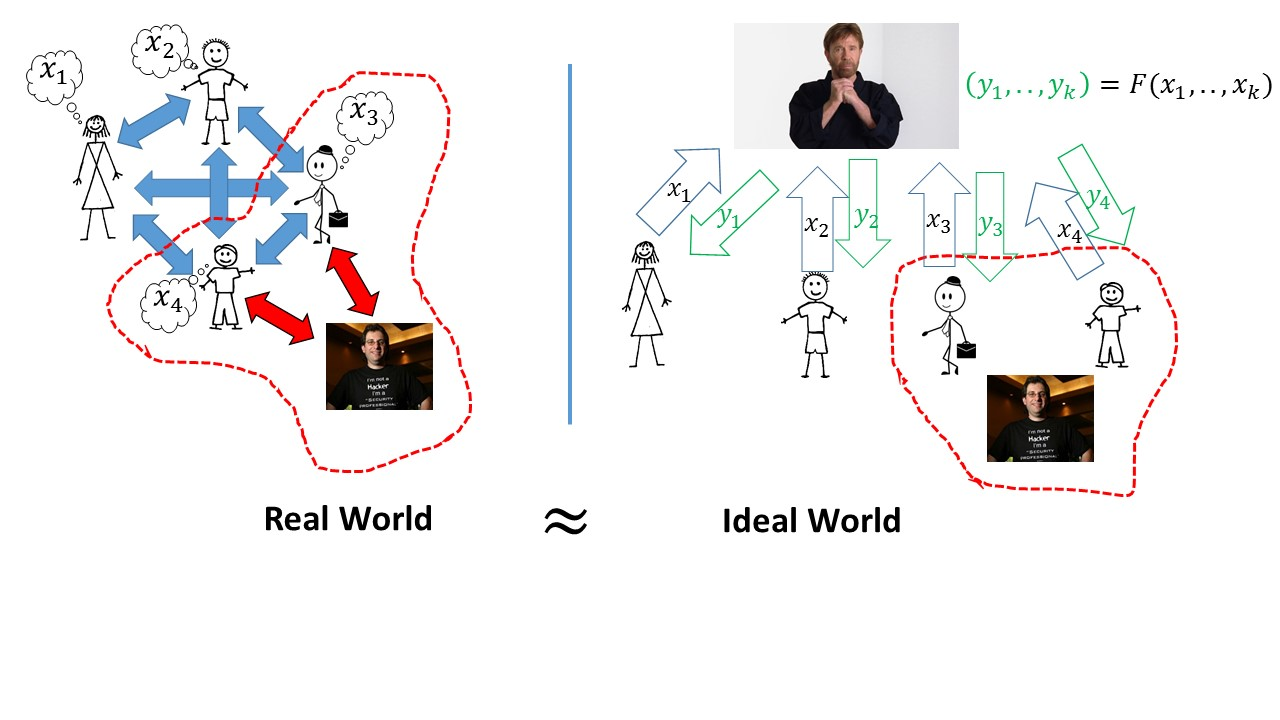
\includegraphics[width=\textwidth, height=0.25\paperheight, keepaspectratio]{../figure/./real-ideal.jpg}
\caption{We define security of a protocol implementing a functionality
\(F\) by stipulating that for every adversary \(A\) that control a
subset of the parties, \(A\)'s view in an actual execution of the
protocol would be indistinguishable from its view in an ideal setting
where all the parties send their inputs to an idealized and perfectly
trusted party, who then computes the outputs and sends it to each
party.}
\label{tmplabelfig}
\end{figure}

Here are some good exercises to make sure you follow the definition:

\begin{itemize}
\item
  Let \(F\) be the two party functionality such that \(F(H\|C,H')\)
  outputs \((1,1)\) if the graph \(H\) equals the graph \(H'\) and \(C\)
  is a Hamiltonian cycle and otherwise outputs \((0,0)\). Prove that a
  protocol for computing \(F\) is a zero knowledge proof\footnote{Actually,
    if we want to be pedantic, this is what's known as a zero knowledge
    \emph{argument} system since soundness is only guaranteed against
    efficient provers. However, this distinction is not important in
    almost all applications.} system for the language of
  Hamiltonicity.\footnote{Our treatment of the input graph \(H\) is an
    instance of a general case. While the definition of a functionality
    only talks about private inputs, it's very easy to include public
    inputs as well. If we want to include some public input \(Z\) we can
    simply have \(Z\) concatenated to all the private inputs (and the
    functionality check that they are all the same, otherwise outputting
    \texttt{error} or some similar result).}
\item
  Let \(F\) be the \(k\)-party functionality that on inputs
  \(x_1,\ldots,x_k \in \{0,1\}\) outputs to all parties the majority
  value of the \(x_i\)'s. Then, in any protocol that securely computes
  \(F\), for any adversary that controls less than half of the parties,
  if at least \(n/2+1\) of the other parties' inputs equal \(0\), then
  the adversary will not be able to cause an honest party to output
  \(1\).
\end{itemize}

\begin{pause} \label[pause]{18-It-is-an-excellent-ide}

It is an excellent idea for you to pause here and try to work out at
least informally these exercises.

\end{pause}

Amazingly, we can obtain such a protocol for \emph{every} functionality:

\hypertarget{MPCthm}{}
\begin{theorem}[Fundamental theorem of cryptography] \label[theorem]{MPCthm}

Under reasonable assumptions\footnote{Originally this was shown under
  the assumption of trapdoor permutations (which can be derived from the
  Factoring or RSA conjectures) but it is known today under a variety of
  other assumptions, including in particular the LWE conjecture.} for
every polynomial-time computable \(k\)-functionality \(F\) there is a
polynomial-time protocol that computes it securely.

\end{theorem}

\cref{MPCthm} was originally proven by Yao in 1982 for the special case
of two party functionalities, and then proved for the general case by
Goldreich, Micali, and Wigderson in 1987. As discussed below, many
variants of this theorem has been shown, and this line of research is
still ongoing.

\subsection{Some comments:}\label{18-Some-comments}

There is in fact not a single theorem but rather many variants of this
fundamental theorem obtained by great many people, depending on the
different security properties desired, as well as the different
cryptographic and setup assumptions. Some of the issues studied in the
literature include the following:

\begin{itemize}
\item
  \textbf{Fairness, guaranteed output delivery:} The definition above
  does not attempt to protect against ``denial of service'' attacks, in
  the sense that the adversary is allowed, even in the ideal case, to
  prevent the honest parties from receiving their outputs.\\
  As mentioned above, without honest majority this is essential for
  simlar reasons to the issue we discussed in
  \href{http://www.boazbarak.org/cs127/chap07_hash_functions.pdf}{our
  lecture on bitcoin} why achieving consensus is hard if there isn't a
  honest majority. When there is an honest majority, we can achieve the
  property of \emph{guaranteed output delivery}, which offers protection
  against such ``denial of service'' attacks. Even when there is no
  guaranteed output delivery, we might want the property of
  \emph{fairness}, whereas we guarantee that if the honest parties don't
  get the output then neither does the adversary. There has been
  extensive study of fairness and there are protocols achieving variants
  on it under various computational and setup assumptions.
\item
  \textbf{Network models:} The current definition assumes we have a set
  of \(k\) parties with known identities with pairwise secure
  (confidential and authenticated) channels between them. Other network
  models studies include broadcast channel, non-private networks, and
  even \href{https://eprint.iacr.org/2007/464}{no authentication}).
\item
  \textbf{Setup assumptions:} The definition does not assume a trusted
  third party, but people have studied different setup assumptions
  including a public key infrastructure, common reference string, and
  more.
\item
  \textbf{Adversarial power:} It turns out that under certain condition,
  it can be possible to obtain secure multiparty computation with
  respect to adversaries that have unbounded computational power (so
  called ``information theoretic security''). People have also studies
  different variants of adversaries including ``honest but curious'' or
  ``passive adversaries'', as well as ``covert'' adversaries that only
  deviate from the protocol if they won't be caught. Other settings
  studied limit the adversary's ability to control parties (e.g., honest
  majority, smaller fraction of parties or particular patterns of
  control, adaptive vs static corruption).
\item
  \textbf{Concurrent compositions:} The definition displayed above are
  for \emph{standalone execution} which is known not to automatically
  imply security with respect to \emph{concurrent composition}, where
  many copies of the same protocol (or different protocols) could be
  executed simultaneously. This opens up all sorts of new
  attacks.\footnote{One example of the kind of issues that can arise is
    the ``grandmasters attack'' whereby someone with no knowledge of
    chess could play two grandmasters simultaneously, relaying their
    moves to one another and thereby guaranteeing a win in at least one
    of the games (or a draw in both).} See
  \href{http://u.cs.biu.ac.il/~lindell/thesis.html}{Yehuda Lindell's
  thesis} (or
  \href{http://u.cs.biu.ac.il/~lindell/LNCSmonograph.html}{this updated
  version}) for more. A very general notion known as ``UC security''
  (which stands for ``Universally Composable'' or maybe ``Ultimate
  Chuck'') has been proposed to achieve security in these settings,
  though at a price of additional setup assumptions, see
  \href{http://www.cs.tau.ac.il/~canetti/materials/ICALP08.pdf}{here}
  and \href{http://eprint.iacr.org/2007/475}{here}.
\item
  \textbf{Communication:} The communication cost for \cref{MPCthm} can
  be proportional to the size of the circuit that computes \(F\). This
  can be a very steep cost, especially when computing over large amounts
  of data. It turns out that we can sometimes avoid this cost using
  fully homomorphic encryption or other techniques.
\item
  \textbf{Efficiency vs.~generality:} While \cref{MPCthm} tells us that
  essentially every protocol problem can be solved \emph{in principle},
  its proof will almost never yield a protocol you actually want to run
  since it has enormous efficiency overhead. The issue of efficiency is
  the biggest reason why secure multiparty computation has so far not
  had a great many practical applications. However, researchers have
  been showing more efficient tailor-made protocols for particular
  problems of interest, and there has been steady progress in making
  those results more practical. See
  \href{http://crypto.biu.ac.il/5th-biu-winter-school}{the slides and
  videos from this workshop} for more.
\end{itemize}

\paragraph{Is multiparty secure computation the end of crypto?} The
notion of secure multiparty computation seems so strong that you might
think that once it is achieved, aside from efficiency issues, there is
nothing else to be done in cryptography. This is very far from the
truth. Multiparty secure computation do give a way to solve a great many
problems in the setting where we have arbitrary rounds of interactions
and unbounded communication, but this is far from being always the case.
As we mentioned before, interaction can sometimes make a
\emph{qualitative} difference (when Alice and Bob are separated by time
rather than space). As we've seen in the discussion of fully homomorphic
encryption, there are also other properties, such as compact
communication, which are not implied by multiparty secure computation
but can make all the difference in contexts such as cloud computing.
That said, multiparty secure computation is an extremely general
paradigm that does apply to many cryptographic problems.

\paragraph{Further reading:} The
\href{http://repository.cmu.edu/cgi/viewcontent.cgi?article=1004\&context=jpc}{survey
of Lindell and Pinkas} gives a good overview of the different variants
and security properties considered in the literature, see also Section 7
in \href{http://www.wisdom.weizmann.ac.il/~oded/foc-sur04.html}{this
survey of Goldreich}. Chapter 6 in
\href{http://www.cs.cornell.edu/courses/cs4830/2010fa/lecnotes.pdf}{Pass
and Shelat's notes} is also a good source.

\section{Example: Second price auction using
bitcoin}\label{18-Example-Second-price-a}

Suppose we have the following setup: an auctioneer wants to sell some
item and run a second-price auction, where each party submits a sealed
bid, and the highest bidder gets the item for the price of the second
highest bid. However, as mentioned above, the bidders do not want the
auctioneer to learn what their bid was, and in general nothing else
other than the identity of the highest bidder and the value of the
second highest bid. Moreover, we might want the payment is via an
electronic currency such as bitcoin, so that the auctioneer not only
gets the information about the winning bid but an actual self-certifying
transaction they can use to get the payment.

Here is how we could obtain such a protocol using secure multiparty
computation:

\begin{itemize}
\item
  We have \(k\) parties where the first party is the auctioneer and
  parties \(2,\ldots,k\) are bidders. Let's assume for simplicity that
  each party \(i\) has a public key \(v_i\) that is associated with some
  bitcoin account.\footnote{As we discussed before, bitcoin doesn't have
    the notion of accounts but rather what we mean by that for each one
    of the public keys, the public ledger contains a sufficiently large
    amount of bitcoins that have been transferred to these keys (in the
    sense that whomever can sign w.r.t. these keys can transfer the
    corresponding coins).} We treat all these keys as the public input.
\item
  The private input of bidder \(i\) is the value \(x_i\) that it wants
  to bid as well as the secret key \(s_i\) that corresponds to their
  public key.
\item
  The functionality only provides an output to the auctioneer, which
  would be the identity \(i\) of the winning bidder as well as a valid
  signature on this bidder transferring \(x\) bitcoins to the key
  \(v_1\) of the auctioneer, where \(x\) is the value of the second
  largest valid bid (i.e., \(x\) equals to the second largest \(x_j\)
  such that \(s_j\) is indeed the private key corresponding to \(v_j\).)
\end{itemize}

It's worthwhile to think about what a secure protocol for this
functionality accomplishes. For example:

\begin{itemize}
\item
  The fact that in the ideal model the adversary needs to choose its
  queries independently means that the adversary cannot get any
  information about the honest parties' bids before deciding on its bid.
\item
  Despite all parties using their signing keys as inputs to the
  protocol, we are guaranteed that no one will learn anything about
  another party's signing key except the single signature that will be
  produced.
\item
  Note that if \(i\) is the highest bidder and \(j\) is the second
  highest, then at the end of the protocol we get a valid signature
  using \(s_i\) on a transaction transferring \(x_j\) bitcoins to
  \(v_1\), despite \(i\) not knowing the value \(x_j\) (and in fact
  never learning the identity of \(j\).) Nonetheless, \(i\) is
  guaranteed that the signature produced will be on an amount not larger
  than its own bid and an amount that one of the other bidders actually
  bid for.
\end{itemize}

I find the ability to obtain such strong notions of security pretty
remarkable. This demonstrates the tremendous power of obtaining
protocols for general functionalities.

\subsection{Another example: distributed and threshold
cryptography}\label{18-Another-example-distri}

It sometimes makes sense to use multiparty secure computation for
\emph{cryptographic computations} as well. For example, there might be
several reasons why we would want to ``split'' a secret key between
several parties, so no party knows it completely.

\begin{itemize}
\item
  Some proposals for \emph{key escrow} (giving government or other
  entity an option for decrypting communication) suggested to split a
  cryptographic key between several agencies or institutions (say the
  FBI, the courts, etc..) so that they must collaborate in order to
  decrypt communication, thus hopefully preventing unlawful access.
\item
  On the other side, a company might wish to split its own key between
  several servers residing in different countries, to ensure not one of
  them is completely under one jurisdiction. Or it might do such
  splitting for technical reasons, so that if there is a break in into a
  single site, the key is not compromised.
\end{itemize}

There are several other such examples. One problem with this approach is
that splitting a cryptographic key is not the same as cutting a 100
dollar bill in half. If you simply give half of the bits to each party,
you could significantly harm security. (For example, it is possible to
recover the full RSA key \href{http://eprint.iacr.org/2008/510.pdf}{from
only \(27\%\) of its bits}).

Here is a better approach, known as
\href{https://en.wikipedia.org/wiki/Secret_sharing}{secret sharing}: To
securely share a string \(s\in\{0,1\}^n\) among \(k\) parties so that
any \(k-1\) of them have no information about it, we choose
\(s_1,\ldots,s_{k-1}\) at random in \(\{0,1\}^n\) and let
\(s_k = s \oplus s_1 \oplus \cdots s_{k-1}\) (\(\oplus\) as usual
denotes the XOR operation), and give party \(i\) the string \(s_i\),
which is known as the \emph{\(i^{th}\) share} of \(s\). Note that
\(s = s_1 \oplus \cdots \oplus s_t\) and so given all \(k\) pieces we
can reconstruct the key. Clearly the first \(k-1\) parties did not
receive any information about \(s\) (since their shares were generated
independent of \(s\)), but the following not-too-hard claim shows that
this holds for \emph{every} set of \(k-1\) parties:

\hypertarget{secretsharinglem}{}
\begin{lemma} \label[lemma]{secretsharinglem}

For every \(s\in\{0,1\}^n\), and set \(T\subseteq [k]\) of size \(k-1\),
we get exactly the same distribution over \((s_1,\ldots,s_k)\) as above
if we choose \(s_i\) for \(i\in T\) at random and set
\(s_t = s \oplus_{i\in T} s_i\) where \(t = [k]\setminus T\).

\end{lemma}

We leave the proof of \cref{secretsharinglem} as an exercise.

Secret sharing solves the problem of protecting the key ``at rest'' but
if we actually want to \emph{use} the secret key in order to sign or
decrypt some message, then it seems we need to collect all the pieces
together into one place, which is exactly what we wanted to avoid doing.
This is where multiparty secure computation comes into play, we can
define a functionality \(F\) taking public input \(m\) and secret inputs
\(s_1,\ldots,s_k\) and producing a signature or decryption of \(m\). In
fact, we can go beyond that and even have the parties sign or decrypt a
message without them knowing what this message is, except that it
satisfies some conditions.

Moreover, secret sharing can be generalized so that a threshold other
than \(k\) is necessary and sufficient to reconstruct the secret (and
people have also studied more complicated access patterns). Similarly
multiparty secure computation can be used to achieve distributed
cryptography with finer access control mechanisms.

\section{Proving the fundamental
theorem:}\label{18-Proving-the-fundamenta}

We will complete the proof of (a relaxed version of) the fundamental
theorem over this lecture and the next one. The proof consists of two
phases:

\begin{enumerate}
\def\labelenumi{\arabic{enumi}.}
\item
  A protocol for the ``honest but curious'' case using fully homomorphic
  encryption.
\item
  A reduction of the general case into the ``honest but curious'' case
  where the adversary follows the protocol precisely but merely attempts
  to learn some information on top of the output that it is ``entitled
  to'' learn. (This reduction is based on zero knowledge proofs and is
  due to Goldreich, Micali and Wigderson)
\end{enumerate}

We note that while fully homomorphic encryption yields a conceptually
simple approach for the second step, it is not currently the most
efficient approach, and rather most practical implementations are based
on the technique known as ``Yao's Garbled Ciruits'' (see
\href{http://u.cs.biu.ac.il/~lindell/efficient-protocols.html}{this
book} or \href{https://eprint.iacr.org/2004/175.pdf}{this paper} or
\href{https://www.cs.uic.edu/pub/Bits/PeterSnyder/Peter_Snyder_-_Garbled_Circuits_WCP_2_column.pdf}{this
survey} ) which in turn is based a notion known as
\href{https://en.wikipedia.org/wiki/Oblivious_transfer}{oblivious
transfer} which can be thought of as a ``baby private information
retrieval'' (though it preceded the latter notion).

We will focus on the case of \emph{two parties}. The same ideas extend
to \(k>2\) parties but with some additional complications.

\section{Malicious to honest but curious reduction}\label{hbctomalred}

We start from the second stage. Giving a reduction transforming a
protocol in the ``honest but curious'' setting into a protocol secure in
the malicious setting. That is, we will prove the following theorem:

\hypertarget{hbctomalthm}{}
\begin{theorem}[Honest-but-curious to malicious security compiler] \label[theorem]{hbctomalthm}

There is a polynomial-time ``compiler'' \(C\) such that for every for
every \(k\) party protocol \((P_1,\ldots,P_k)\) (where all \(P_i\)'s are
polynomial-time computable potentially randomized strategies), if we let
\((\tilde{P}_1,\ldots,\tilde{P}_k) = C(P_1,\ldots,P_k)\) will be a
\(k\)-tuple polynomial-time computable strategies and moreover if
\((P_1,\ldots,P_k)\) was a protocol for computing some (potentially
randomized) functionality \(F\) secure with respect to
honest-but-curious adversaries, then
\((\tilde{P}_1,\ldots,\tilde{P}_k)\) is a protocol for computing the
same \(F\) secure with respect to \emph{malicious} adversaries.

\end{theorem}

The remainder of this section is devoted to the proof of
\cref{hbctomalthm}. For ease of notation we will focus on the \(k=2\)
case, where there are only two parties (``Alice'' and ``Bob'') although
these techniques generalize to arbitrary number of parties \(k\). Note
that a priori, it is not obvious at all that such a compiler should
exist. In the ``honest but curious'' setting we assume the adversary
follows the protocol to the letter. Thus a protocol where Alice gives
away all her secrets to Bob if he merely
\href{https://xkcd.com/424/}{asks her to do so politely} can be secure
in the ``honest but curious'' setting if Bob's instructions are not to
ask. More seriously, it could very well be that Bob has an ability to
deviate from the protocol in subtle ways that would be completely
undetectable but allow him to learn Alice's secrets. Any transformation
of the protocol to obtain security in the malicious setting will need to
rule out such deviations.

The main idea is the following: we do the compilation one party at a
time - we first transform the protocol so that it will remain secure
even if Alice tries to cheat, and then transform it so it will remain
secure even if Bob tries to cheat. Let's focus on Alice. Let's imagine
(without loss of generality) that Alice and Bob alternate sending
messages in the protocol with Alice going first, and so Alice sends the
odd messages and Bob sends the even ones. Lets denote by \(m_i\) the
message sent in the \(i^{th}\) round of the protocol. Alice's
instructions can be thought of as a sequence of functions
\(f_1,f_3,\cdots,f_t\) (where \(t\) is the last round in which Alice
speaks) where each \(f_i\) is an efficiently computable function mapping
Alice's secret input \(x_1\), (possibly) her random coins \(r_1\), and
the transcript of the previous messages \(m_1,\ldots,m_{i-1}\) to the
next message \(m_i\). The functions \(\{ f_i \}\) are publicly known and
part of the protocol's instructions. The only thing that Bob doesn't
know is \(x_1\) and \(r_1\). So, our idea would be to change the
protocol so that after Alice sends the message \(i\), she \emph{proves}
to Bob that it was indeed computed correctly using \(f_i\). If \(x_1\)
and \(r_1\) weren't secret, Alice could simply send those to Bob so he
can verify the computation on his own. But because they are (and the
security of the protocol could depend on that) we instead use a
\emph{zero knowledge proof}.

Let's assume for starters that Alice's strategy is \emph{deterministic}
(and so there is no random tape \(r_1\)). A first attempt to ensure she
can't use a malicious strategy would be for Alice to follow the message
\(m_i\) with a zero knowledge proof that there exists some \(x_1\) such
that \(m_i=f(x_1,m_1,\ldots,m_{i-1})\). However, this will actually not
be secure - it is worth while at this point for you to pause and think
if you can understand the problem with this solution.

\begin{pause} \label[pause]{18-Really-please-stop-and}

Really, please stop and think why this will not be secure.

\end{pause}

\newpage

\begin{pause} \label[pause]{18-Did-you-stop-and-think}

Did you stop and think?

\end{pause}

The problem is that at every step Alice proves that there exists
\emph{some} input \(x_1\) that can explain her message but she doesn't
prove that it's \emph{the same input for all messages}. If Alice was
being truly honest, she should have picked her input once and use it
throughout the protocol, and she could not compute the first message
according to the input \(x_1\) and then the third message according to
some input \(x'_1 \neq x_1\). Of course we can't have Alice reveal the
input, as this would violate security. The solution is for Alice to
\emph{commit} in advance to the input. We have seen commitments before,
but let us now formally define the notion:

\hypertarget{commitmentdef}{}
\begin{definition}[Commitment scheme] \label[definition]{commitmentdef}

A \emph{commitment scheme} for strings of length \(\ell\) is a two party
protocol between the \emph{sender} and \emph{receiver} satisfying the
following:

\begin{itemize}
\item
  \textbf{Hiding (sender's security):} For every two sender inputs
  \(x,x' \in \{0,1\}^\ell\), and no matter what efficient strategy the
  receiver uses, it cannot distinguish between the interaction with the
  sender when the latter uses \(x\) as opposed to when it uses \(x'\).
\item
  \textbf{Binding (reciever's security):} No matter what (efficient or
  non efficient) strategy the sender uses, if the reciever follows the
  protocol then with probability \(1-negl(n)\), there will exist at most
  a single string \(x\in\{0,1\}^\ell\) such that the transcript is
  consistent with the input \(x\) and some sender randomness \(r\).
\end{itemize}

\end{definition}

That is, a commitment is the digital analog to placing a message in a
sealed envelope to be opened at a later time. To commit to a message
\(x\) the sender and reciever interact according to the protocol, and to
\emph{open} the commitment the sender simply sends \(x\) as well as the
random coins it used during the commitment phase. The variant we defined
above is known as \emph{computationally hiding and statistically
binding}, since the sender's security is only guaranteed against
efficient receivers while the binding property is guaranteed against all
senders. There are also statistically hiding and computationally binding
commitments, though it can be shown that we need to restrict to
efficient strategies for at least one of the parties.

We have already seen a commitment scheme before (due to Naor): the
receiver sends a random \(z\leftarrow_R\{0,1\}^{3n}\) and the sender
commits to a bit \(b\) by choosing a random \(s\in\{0,1\}^n\) and
sending \(y = \ensuremath{\mathit{PRG}}(s)+ bz (\mod 2)\) where
\(\ensuremath{\mathit{PRG}}:\{0,1\}^n\rightarrow\{0,1\}^{3n}\) is a
pseudorandom generator. It's a good exercise to verify that it satisfies
the above definitions. By running this protocol \(\ell\) times in
parallel we can commit to a string of any polynomial length.

We can now describe the transformation ensuring the protocol is secure
against a malicious Alice in full, for the case that that the original
strategy of Alice is \emph{deterministic} (and hence uses no random
coins)

\begin{itemize}
\item
  Initially Alice and Bob engage in a commitment scheme where Alice
  commits to her input \(x_1\). Let \(\tau\) be the transcript of this
  commitment phase and \(r_{com}\) be the randomness Alice used during
  it.\footnote{Note that even though we assumed that in the original
    honest-but-curious protocol Alice used a deterministic strategy, we
    will transform the protocol into one in which Alice uses a
    randomized strategy in both the commitment and zero knowledge
    phases.}
\item
  For \(i=1,2,\ldots\):

  \begin{itemize}
  \item
    If \(i\) is even then Bob sends \(m_i\) to Alice
  \item
    If \(i\) is odd then Alice sends \(m_i\) to Bob and then they engage
    in a zero knowledge proof that there exists \(x_1,r_{com}\) such
    that (1) \(x_1,r_com\) is consistent with \(\tau\), and (2)
    \(m_i = f(x_1,m_1,\ldots,m_{i-1})\). The proof is repeated a
    sufficient number of times to ensure that if the statement is false
    then Bob rejects with \(1-negl(n)\) probability.
  \item
    If the proof is rejected then Bob aborts the protocol.
  \end{itemize}
\end{itemize}

We will not prove security but will only sketch it here, see
\href{http://www.nowpublishers.com/article/Details/TCS-001}{Section
7.3.2 in Goldreich's survey} for a more detailed proof:

\begin{itemize}
\item
  To argue that we maintain security for \emph{Alice} we use the zero
  knowledge property: we claim that Bob could not learn anything from
  the zero knowledge proofs precisely because he could have simulated
  them by himself. We also use the hiding property of the commitment
  scheme. To prove security formally we ~need to show that whatever Bob
  learns in the modified protocol, he could have learned in the original
  protocol as well. We do this by \emph{simulating} Bob by replacing the
  commitment scheme with commitment to some random junk instead of
  \(x_1\) and the zero knowledge proofs with their simulated version.
  The proof of security requires a hybrid argument, and is again a good
  exercise to try to do it on your own.
\item
  To argue that we maintain security for \emph{Bob} we use the binding
  property of the commitment scheme as well as the soundness property of
  the zero knowledge system. Once again for the formal proof we need to
  show that we could transform any potentially malicious strategy for
  Alice in the modified protocol into an ``honest but curious'' strategy
  in the original protocol (also allowing Alice the ability to abort the
  protocol). It turns out that to do so, it is not enough that the zero
  knowledge system is sound but we need a stronger property known as a
  \emph{proof of knowledge}. We will not define it formally, but roughly
  speaking it means we can transform any prover strategy that convinces
  the verifier that a statement is true with non-negligible probability
  into an algorithm that outputs the underlying secret (i.e., \(x_1\)
  and \(r_com\) in our case). This is crucial in order to trasnform
  Alice's potentially malicious strategy into an honest but curious
  strategy.
\end{itemize}

We can repeat this transformation for Bob (or Charlie, David, etc.. in
the \(k>2\) party case) to transform a protocol secure in the honest but
curious setting into a protocol secure (allowing for aborts) in the
malicious setting.

\subsection{Handling probabilistic
strategies:}\label{18-Handling-probabilistic}

So far we assumed that the original strategy of Alice in the honest but
curious is deterministic but of course we need to consider probabilistic
strategies as well. One approach could be to simply think of Alice's
random tape \(r\) as part of her secret input \(x_1\). However, while in
the honest but curious setting Alice is still entitled to freely choose
her own input \(x_1\), she is not entitled to choose the random tape as
she wishes but is supposed to follow the instructions of the protocol
and choose it uniformly at random. Hence we need to use a \emph{coin
tossing protocol} to choose the randomness, or more accurately what's
known as a ``coin tossing in the well'' protocol where Alice and Bob
engage in a coin tossing protocol at the end of which they generate some
random coins \(r\) that only Alice knows but Bob is still guaranteed
that they are random. Such a protocol can actually be achieved very
simply. Suppose we want to generate \(m\) coins:

\begin{itemize}
\tightlist
\item
  Alice selects \(r'\leftarrow_R\{0,1\}^m\) at random and engages in a
  \emph{commitment protocol} to commit to \(r'\).
\item
  Bob selects \(r'' \leftarrow_R\{0,1\}^m\) and sends it to Alice in the
  clear.
\item
  The result of the coin tossing protocol will be the string
  \(r=r'\oplus r''\).
\end{itemize}

Note that Alice knows \(r\). Bob doesn't know \(r\) but because he chose
\(r''\) \emph{after} Alice committed to \(r'\) he knows that it must be
fully random regardless of Alice's choice of \(r'\). It can be shown
that if we use this coin tossing protocol at the beginning and then
modify the zero knowledge proofs to show that
\(m_i=f(x_1,r_1,m_1,\ldots,m_{i-1})\) where \(r\) is the string that is
consistent with the transcript of the coin tossing protocol, then we get
a general transformation of an honest but curious adversary into the
malicious setting.

The notion of multiparty secure computation - defining it and achieving
it - is quite subtle and I do urge you to read some of the other
references listed above as well. In particular, the slides and videos
from the
\href{https://cyber.biu.ac.il/event/the-1st-biu-winter-school/}{Bar Ilan
winter school on secure computation and efficiency}, as well as the ones
from the
\href{https://cyber.biu.ac.il/event/the-5th-biu-winter-school/}{winter
school on advances in practical multiparty computation} are great
sources for this and related materials.
